% Fig. 3 — Confusion matrix C4 (normalized by row)
\begin{figure}[t]
\centering
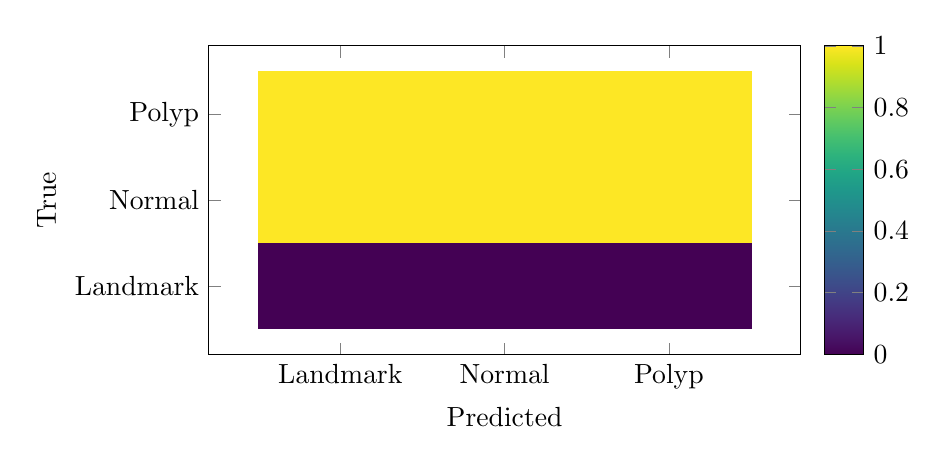
\begin{tikzpicture}
\begin{axis}[
  width=0.75\linewidth,
  height=5.5cm,
  xlabel={Predicted},
  ylabel={True},
  xtick=data,
  ytick=data,
  xticklabels={Landmark,Normal,Polyp},
  yticklabels={Landmark,Normal,Polyp},
  colormap/viridis,
  colorbar,
  point meta min=0,
  point meta max=1,
  axis on top,
]
\addplot[
  matrix plot*,
  mesh/cols=3,
  mesh/rows=3,
] table[meta=z] {
x y z
0 0 0.931
1 0 0.024
2 0 0.046
0 1 0.007
1 1 0.990
2 1 0.003
0 2 0.124
1 2 0.047
2 2 0.828
};
\end{axis}
\end{tikzpicture}
\caption{Row-normalized confusion matrix for C4 on test ($n=1433$). Primary clinical concern: polyp recall 82.8\%.}
\label{fig:confusion}
\end{figure}
